\documentclass{beamer}
\usepackage[utf8]{inputenc}
\usepackage{tikz}
\usepackage{hyperref}
\usetheme{Madrid}
\usecolortheme{default}
\usetikzlibrary{arrows.meta, positioning}
\usepackage{listings}
\usepackage{xcolor}
\usepackage[]{biblatex}
\usepackage[linesnumbered,ruled,vlined]{algorithm2e}


\bibliography{citations}
% comment a region
% Put all your custom macros here
\usepackage{xspace}
\newcommand{\cmnt}[1]{}
\newcommand{\ignore}[1]{}
\newcommand{\remove}[1]{}

% a word should not be broken across lines
\newcommand{\nosplit}{\linebreak}

% no hyphenation
\def\nohyphens{\hyphenpenalty=10000\exhyphenpenalty=10000}

% ~ character
\newcommand{\tilda}{\symbol{126}}

% useful mathematical symbols

\newcommand{\ang}[1]{\langle #1 \rangle}
\newcommand{\Ang}[1]{\Big\langle #1 \Big\rangle}
\newcommand{\ceil}[1]{\lceil #1 \rceil}
\newcommand{\floor}[1]{\lfloor #1 \rfloor}
% \newtheorem{definition}{Definition}

% quantifiers
\newcommand{\myforall}[3]{\ang{\forall \: #1 : #2 : #3 }}
\newcommand{\myexists}[3]{\ang{\exists \: #1 : #2 : #3 }}
\newcommand{\mynexists}[3]{\ang{\nexists \: #1 : #2 : #3 }}
\newcommand{\Myforall}[3]{\Ang{\forall \: #1 : #2 : #3 }}
\newcommand{\Myexists}[3]{\Ang{\exists \: #1 : #2 : #3 }}
\newcommand{\Mynexists}[3]{\Ang{\nexists \: #1 : #2 : #3 }}


% for formally defining a notion
% \newcommand{\defined}{\;\;\stackrel{\triangle}{=}\;\;}
\newcommand{\defined}{\;\;\triangleq\;\;}


% mathematical implications

%\renewcommand{\implies}{\Rightarrow}
\newcommand{\follows}{\Leftarrow}

% miscellaenous
\newcommand{\myspace}{\hspace*{0.0in}}
\newcommand{\halflinespacing}{\vspace*{0.5em}}
\newcommand{\greaterlinespacing}{\vspace*{0.75em}}

%/commands for personal comments
\newcommand {\spnote}[1] {\todo[inline,size=\footnotesize,color=yellow!20]{Sathya: #1}}
\newcommand {\manasnote}[1] {\todo[inline,size=\footnotesize,color=yellow!20]{Manas: #1}}
\newcommand {\cgnote}[1] {\todo[inline,size=\footnotesize,color=yellow!20]{Chryssis: #1}}

\newcommand {\spcolor}[1] {\textcolor{green}{#1}}
\newcommand {\spdiff}[1] {\textcolor{orange}{#1}}
\newcommand {\mpcolor}[1] {\textcolor{blue}{#1}}

%%%%%%%%%%%%%%%%%%%%%%%%%%%%%%%%%%%%%%%%%%%%%%%%%%%%%%%%%%%%%%%%%%%%%%%%%%%%%%%%%%%%%%%%%%%%%%

%% various theorem environments
%% Commented out because they are already defined in llncs file %%
%% Decommented out because they are not defined in sigplan class %%

% \newtheorem{theorem}{Theorem}
%\renewcommand{\thetheorem}{\arabic{theorem}}
% \newtheorem{lemma}{Lemma}

%\newtheorem{lemma}[theorem]{Lemma}
% \newtheorem{corollary}{Corollary}
%\newtheorem{proposition}[theorem]{Proposition}
%\newtheorem{property}[theorem]{Property}
%\newtheorem{definition}[theorem]{Definition}

%\renewtheorem{property}[theorem]{Property}

% \newtheorem{definition}{Definition}
%\renewcommand{\thedefinition}{\arabic{definition}}

%\newtheorem{property}{Property}
%\renewcommand{\theproperty}{\arabic{property}}

% \newtheorem{observation}[lemma]{Observation}
%\renewcommand{\theobservation}{\arabic{observation}}

%\newtheorem{example}{Example}
%\renewcommand{\theexample}{\arabic{example}}

%\newtheorem{assume}{Assumption}
%\renewcommand{\theassume}{\arabic{assume}}

%\newtheorem{remark}{Remark}
%\renewcommand{\theremark}{\arabic{remark}}

%\newtheorem{axiom}[theorem]{Proposition}
%\renewcommand{\theaxiom}{\arabic{axiom}}

%\newtheorem{invariant}[theorem]{Invariant}

%\renewcommand{\theequation}{\arabic{equation}}

%-----------------Theorem Notations Defined by Petr ---------------------------------------------------------------------------------------------------------
%% Defined by Petr
\newtheorem{requirement}{Requirement}
%------------------------------------------------------------------------------------------------------------------------------

% \newtheorem{definition}{Definition}

% various references
\newcommand{\chapref}[1]{Chapter~\ref{chap:#1}}
\newcommand{\secref}[1]{Section~\ref{sec:#1}}
\newcommand{\figref}[1]{Fig.~\ref{fig:#1}}
\newcommand{\tabref}[1]{Table~\ref{tab:#1}}
\newcommand{\stref}[1]{step~\ref{step:#1}}
\newcommand{\thmref}[1]{Theorem~\ref{thm:#1}}
\newcommand{\lemref}[1]{Lemma~\ref{lem:#1}}
%\newcommand{\corref}[1]{Corollary~\ref{cor:#1}}
\newcommand{\axmref}[1]{Proposition~\ref{axm:#1}}
\newcommand{\defref}[1]{Definition~\ref{def:#1}}
\newcommand{\eqnref}[1]{Eqn(\ref{eq:#1})}
\newcommand{\eqvref}[1]{Equivalence~(\ref{eqv:#1})}
\newcommand{\ineqref}[1]{Inequality~(\ref{ineq:#1})}
%\newcommand{\invref}[1]{(\ref{inv:#1})}
\newcommand{\exref}[1]{Example~\ref{ex:#1}}
\newcommand{\propref}[1]{Property~\ref{prop:#1}}
\newcommand{\obsref}[1]{Observation~\ref{obs:#1}}
\newcommand{\asmref}[1]{Assumption~\ref{asm:#1}}
\newcommand{\thref}[1]{Thread~\ref{th:#1}}
\newcommand{\trnref}[1]{Transaction~\ref{trn:#1}}
\newcommand{\grfref}[1]{Graph~\ref{graph:#1}}

\newcommand{\lineref}[1]{Line~\ref{lin:#1}}
\newcommand{\algoref}[1]{{Algorithm \ref{alg:#1}}}
\newcommand{\subsecref}[1]{SubSection~\ref{subsec:#1}}
\newcommand{\subsubsecref}[1]{SubSubSection~\ref{subsubsec:#1}}

\newcommand{\apnref}[1]{Appendix~\ref{apn:#1}}
\newcommand{\invref}[1]{Invariant~\ref{inv:#1}}

\newcommand{\specref}[1] {Specification~\ref{spec:#1}}

\newcommand{\Chapref}[1]{Chapter~\ref{chap:#1}}
\newcommand{\Secref}[1]{Section~\ref{sec:#1}}
\newcommand{\Figref}[1]{Figure~\ref{fig:#1}}
\newcommand{\Tabref}[1]{Table~\ref{tab:#1}}
\newcommand{\Stref}[1]{Step~\ref{step:#1}}
\newcommand{\Thmref}[1]{Theorem~\ref{thm:#1}}
\newcommand{\Lemref}[1]{Lemma~\ref{lem:#1}}
\newcommand{\Corref}[1]{Corollary~\ref{cor:#1}}
\newcommand{\Axmref}[1]{Proposition~\ref{axm:#1}}
\newcommand{\Defref}[1]{Definition~\ref{def:#1}}
\newcommand{\Eqref}[1]{(\ref{eq:#1})}
\newcommand{\Eqvref}[1]{Equivalence~(\ref{eqv:#1})}
\newcommand{\Ineqref}[1]{Inequality~(\ref{ineq:#1})}
\newcommand{\Exref}[1]{Example~\ref{ex:#1}}
\newcommand{\Propref}[1]{Property~\ref{prop:#1}}
\newcommand{\Obsref}[1]{Observation~\ref{obs:#1}}
\newcommand{\Asmref}[1]{Assumption~\ref{asm:#1}}
\newcommand{\Specref}[1]{Specification~\ref{spec:#1}}

\newcommand{\Lineref}[1]{Line~\ref{lin:#1}}
\newcommand{\Algoref}[1]{{\sf Algo$_{\ref{algo:#1}}$}}

\newcommand{\Apnref}[1]{Section~\ref{apn:#1}}
\newcommand{\Invref}[1]{Invariant~\ref{inv:#1}}
\newcommand{\Grfref}[1]{Graph~\ref{trn:#1}}


% environment for writing a proof

\newcommand{\proofsketch}[1][]{\noindent{\bf\boldmath
                         P\hspace{-0.25ex}roof~Sketch{#1}\/:\unboldmath}\hspace*{0.5em}}


\newcommand{\theqed}{$\Box$}

%\newcommand{\qed}{\hspace*{\fill}\theqed\\\vspace*{-0.5em}}

% In case the proof is immediately followed by the start of a new section

\newcommand{\nsqed}{\hspace*{\fill} \theqed}


% End of example

\newcommand{\eoe}{\qed}

% Renews the footnote command
%\renewcommand{\thefootnote}{\alph{footnote}}

\def\Nomega{\ensuremath{\neg\Omega}}
\def\Vomega{\ensuremath{\overrightarrow{\Omega}}}

\newcommand{\myparagraph}[1]{\vspace{1mm}\noindent\textbf{#1}}

%------------------------------------------------------------------------------------------------------------------
% Definitions for Weak Consistency paper
%------------------------------------------------------------------------------------------------------------------

\newcommand{\op} {operation\xspace}
\newcommand{\termop} {terminal operation\xspace}

\newcommand{\sble} {serializable\xspace}
\newcommand{\sbty} {serializability\xspace}
\newcommand{\lble} {linearizable\xspace}
\newcommand{\lbty} {linearizability\xspace}

\newcommand{\wf} {wait-free\xspace}

\newcommand{\CAS} {\textit{CAS}\xspace}
\newcommand{\mCAS} {\textit{mCAS}\xspace}
\newcommand{\cas} {CAS\xspace}

\newcommand{\cc} {correctness-criterion\xspace}

\newcommand{\rs}{rset\xspace}
\newcommand{\ws}{wset\xspace}


%\newcommand{\Fwrite}{\SetKwFunction{Fwrite}{ABCAS-append}}
%\newcommand{\Fview}{\SetKwFunction{Fview}{ABCAS-read}}

\newcommand{\Fwrite}{{\tt StickyCAS-append}\xspace}
\newcommand{\Fview}{{\tt StickyCAS-read}\xspace}
\newcommand{\BVCAS}{StickyCAS\xspace}
\newcommand{\bvcas}{StickyCAS\xspace}
\newcommand{\abcas}{StickyCAS\xspace}
%\Fwrite{}
%\Fview{}

\newcommand{\Skey} {Worm}
\newcommand{\skey} {worm}
\newcommand{\ie}{\textit{i.e., }}


\newcommand{\mth} {method\xspace}

\newcommand{\cons} {SM-ByzCons}
\newcommand{\sch} {scheduler\xspace}

\newcommand{\sbc} {Strong Byzantine Consensus\xspace}
\newcommand{\cvbc} {Common-value Byzantine Consensus\xspace}
\newcommand{\wbc} {Weak Byzantine Consensus\xspace}
%------------------------------------------------------------
%This block of code defines the information to appear in the
%Title page
\title[Byz Consensus GPU]
{Byzantine-Tolerant Consensus in GPU-Inspired Shared Memory}

\author[UCY, IITH]{}

\date[EURO-PAR 2025]{%
\vspace{-5em} 
\begin{figure}
\centering 
\includegraphics[height=1cm]{images.png} \end{figure}
Authors: \\
Chryssis Georgiou, University of Cyprus, Cyprus\\
Manaswini Piduguralla, IIT Hyderabad, India\\
\textbf{Sathya Peri}, IIT Hyderabad, India\\
29 August 2025\\
\vspace{2em}
% --- two images side by side ---
\begin{tabular}{cc}
    
\includegraphics[height=1cm]{UCY.png} &
    
\includegraphics[height=1cm]{iith.png} \\
\end{tabular}
}
    







%End of title page configuration block
%------------------------------------------------------------



%------------------------------------------------------------
%The next block of commands puts the table of contents at the 
%beginning of each section and highlights the current section:

\AtBeginSection[]
{
  \begin{frame}
    \frametitle{Table of Contents}
    \tableofcontents[currentsection]
  \end{frame}
}
%------------------------------------------------------------
% \AtBeginSection[]
% {
%     \begin{frame}
%         \frametitle{Table of Contents}
%         \tableofcontents[currentsection]
%     \end{frame}
% }

\begin{document}

%The next statement creates the title page.
\frame{\titlepage}


%---------------------------------------------------------
%This block of code is for the table of contents after
%the title page
\begin{frame}
\frametitle{Table of Contents}
\tableofcontents
\end{frame}
%---------------------------------------------------------
\section{Research Objective}
%---------------------------------------------------------

\begin{frame}
\frametitle{Research Objective}
Agreement among multiple parties is a fundamental problem in distributed computing  for a wide range of applications \footfullcite{kshemkalyani:book:2011}.
\vspace{1mm}
\begin{itemize}
\item GPUs have evolved from graphics to general-purpose parallel computation.
  \item Their SIMT\footnote{Single Instruction Multiple Threads} execution model and warp-based scheduling differ fundamentally from CPUs.
  \item We aim to explore fundamental problems of distributed computing in a General Purpose GPU (GPGPU) architecture.
\end{itemize}
\end{frame}




%---------------------------------------------------------
\section{Background}
%---------------------------------------------------------

\begin{frame}{The GPU Architecture}
\begin{itemize}
  \item Streaming Multiprocessors (SMs) host many simple cores.
  \item Threads are organized into \textbf{warps} (typically 32) executing in lock-step.
  \item Warp scheduler selects which warp executes in each cycle.
\end{itemize}

\begin{figure}[t]
\centering
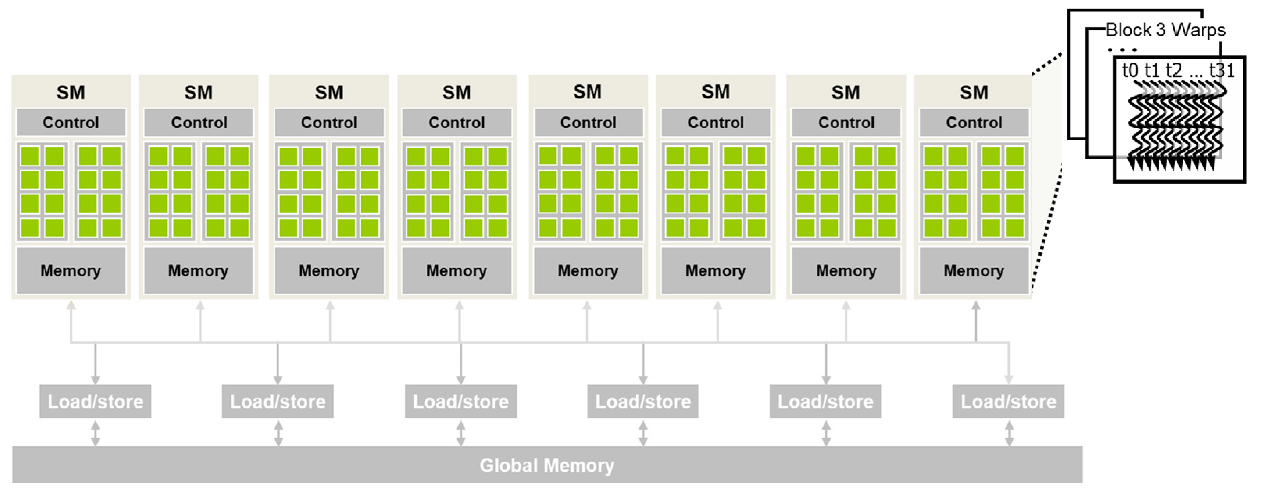
\includegraphics[scale=0.35]{gpuArch.png}
\caption{Illustration of CUDA-capable GPU Architecture\footfullcite{david+:PMPP:science:2017}}
\label{fig:gpuArch}
\end{figure}    
\end{frame}

\begin{frame}{SIMT and Warp Scheduling}
\begin{columns}[T] % align columns at top
  \begin{column}{0.5\textwidth}
    \begin{itemize}
      \item \textbf{SIMT}: Single Instruction, Multiple Threads 
      \item Within a warp: synchronous; across warps: asynchronous.
      \item Warps proceed as the scheduler issues a small, fixed number of instructions per cycle.
    \end{itemize}
  \end{column}

  \begin{column}{0.5\textwidth}
    \begin{figure}
      \centering
      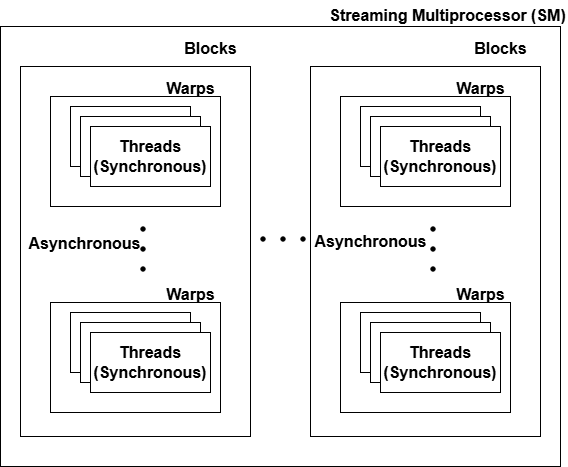
\includegraphics[width=\linewidth]{gpuHier.png}
      \caption{Illustration of GPU Hierarchy}
      \label{fig:GPU-hier}
    \end{figure}
  \end{column}
\end{columns}
\end{frame}

\begin{frame}{Why Byzantine consensus in GPUs}
\begin{itemize}
  \item Multi-tenant GPU setups (e.g., MPS) and fairness in HPC clusters, fault-tolerant resource usage~\footfullcite{Weaver+:SC24:2024} motivated us to investigate consensus.
  \item GPUs show higher susceptibility to hardware errors than CPUs (e.g., transient bit flips)\footfullcite{CiniYalcin:GPU-CPU:ACMSurvey:2020}.
  \item Software malfunctions can lead to silent or inconsistent failures in GPU workloads.
  \item Byzantine model is well-suited for unpredictable failures, as it can provide correctness guarantees even in the presence of arbitrary faults.
\end{itemize}
\end{frame}


%---------------------------------------------------------
\section{Proposed System Model}
%---------------------------------------------------------


\begin{frame}{The GPU-Inspired Shared Memory Model}
\begin{itemize}
  \item System consists of a static set of $n$ processes: $P_1, P_2, \dots, P_n$.
  \item These processes correspond to threads of \textbf{a block} in a Streaming Multiprocessor (SM).
  \item Processes are grouped into warps of \textbf{size} $\boldsymbol{p}$, total $\boldsymbol{\lceil n/p \rceil}$ warps.  
  \item Focus of this work: single block of a single SM (circled).
\end{itemize}
\vspace{-1em}
\begin{figure}[t]
\centering
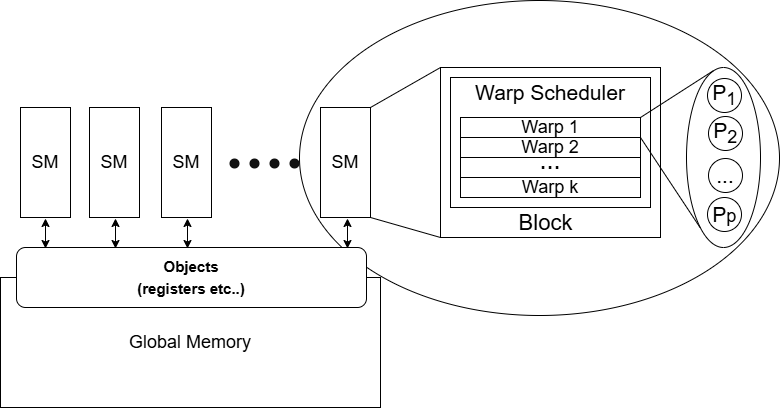
\includegraphics[scale=0.25]{BYZmodel.png}
\caption{Illustration of the system model}
\vspace{-2em}
\label{fig:SysModel}
\end{figure}
\end{frame}

\begin{frame}{Warp Scheduler}
\begin{itemize}
  \item Hardware scheduler maps warps to cores~\footfullcite{Ogier:book:2013}.
  \item Processes can only be activated by the scheduler.
  \item Byzantine threads cannot bypass or impersonate the scheduler.
  \item We assume \textbf{fair scheduling}~\footfullcite{wong:SIGOPS:2008}$^,$\footfullcite{pabla:linux:2009}:
    \begin{itemize}
      \item Each process eventually gets a chance to execute.
      \item Scheduler itself is not Byzantine.
    \end{itemize}
\end{itemize}
\end{frame}




\begin{frame}{Phase-Based Computation}
\begin{itemize}
  \item Computation proceeds in synchronized \textbf{phases}.
  \item One warp ($p$ processes) is scheduled per phase.
  \item Within a phase:
    \begin{itemize}
      \item Processes in the warp execute synchronously in lock-step.
    \end{itemize}
  \item Across different warps: execution is asynchronous.
\end{itemize}

\begin{figure} 
\centering
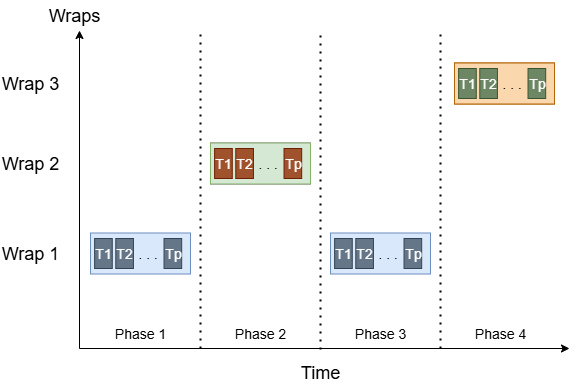
\includegraphics[width=0.45\linewidth]{phase-based-execution.png} 
\vspace{-1em}\caption{Illustration of Phase Based Execution.} \label{fig:phase}
\end{figure}
\end{frame}

\begin{frame}{Failure Model}
\begin{itemize}
  \item We consider \textbf{Byzantine failures}~\footfullcite{ByzGens}.
  \item Up to $f<n$ processes may be corrupted.
  \item Faulty processes:
    \begin{itemize}
      \item May deviate arbitrarily from the protocol.
      \item Cannot impersonate another process or exceed phase latency.
    \end{itemize}
  \item Correct processes follow the protocol and take infinitely many steps.
  \item A protocol tolerating up to $f$ Byzantine processes is called \textit{$f$-resilient}.
\end{itemize}
\end{frame}


%---------------------------------------------------------
\section{Byzantine Consensus}
%---------------------------------------------------------


%------------------------------------------------
\begin{frame}{Introduction to Byzantine Consensus}
\begin{itemize}
  \item Agreement among multiple parties is a fundamental problem in distributed computing~\footfullcite{kshemkalyani:book:2011}.
  \item Recently, there has been increased emphasis on \textbf{Byzantine fault-tolerant shared objects.}~\footfullcite{CKDISC2021}
  \item Consensus: $n$ processes propose values and must agree on a single value.
  \item Different variants exist depending on the validity property.
\end{itemize}
\end{frame}

%------------------------------------------------
%------------------------------------------------
\begin{frame}{Types of Byzantine Consensus Considered} 
% \vspace{-28em}
\begin{itemize} \item In this work, we consider: 

\begin{enumerate} 
\item Strong Byzantine Consensus (SBC)~\footfullcite{Malkhi+:DC:2003} 
\item Common-Value Byzantine Consensus (CVBC)~\footfullcite{attie:IPL:2002} 
\item Weak Byzantine Consensus (WBC)$^{11}$
\end{enumerate} 
\end{itemize} 
\begin{figure} 
\centering
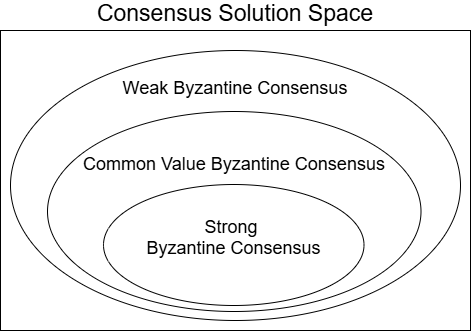
\includegraphics[width=0.35\linewidth]{ByzSolSpace.png} 
\vspace{-1em}\caption{Illustration of Consensus Solution Space.} \label{fig:ByzSol}
\end{figure}

\end{frame}

%------------------------------------------------
\begin{frame}{Strong Byzantine Consensus (SBC)}
\begin{definition}[\sbc] 
	Given $n$ processes, up to $f<n$ faulty, and $V$ is the set of all proposed values, $V_c \subseteq V$ the set of values proposed by correct processes, the following must hold:
	\begin{itemize}
		\item \textbf{Termination: } Every correct process must eventually decide.
		\item \textbf{Agreement: } All correct processes decide the same value $v_f$.
		\item \textbf{Strong Validity: } The decision must be a value proposed by at least one correct process (\ie $v_f \in V_c$).
	\end{itemize}
\end{definition}
{
\small
\textbf{Common-Value Byzantine Consensus (CVBC):} Validity:  If $V_c=\{v\}$, then $v_f = v$.\\


\textbf{Weak Byzantine Consensus (WBC):}Validity: $v_f \in V$.
}
\end{frame}

%------------------------------------------------
% \begin{frame}{Common-Value Byzantine Consensus (CVBC)}
% \begin{definition}[\cvbc] 
% 	Given $n$ processes, up to $f<n$ faulty, and correct values $V_c$, the following must hold:
% 	\begin{itemize}
% 		\item \textbf{Termination: } Every correct process must eventually decide.
% 		\item \textbf{Agreement: } All correct processes decide the same value.
% 		\item \textbf{Common Validity: } If $V_c=\{v\}$, then $v$ must be the consensus value.
% 	\end{itemize}
% \end{definition}
% \end{frame}



%---------------------------------------------------------
\section{Proposed Solution}
%---------------------------------------------------------


\begin{frame}{Proposed Solution}
\begin{itemize}
  \item We propose a novel shared object, called \textbf{\BVCAS} (Sticky Compare\&Swap).
  \item Inspired by sticky bits~\footfullcite{Malkhi+:DC:2003}, but generalized for \textit{multi-valued consensus}.
  \item Acts as a non-corruptible shared memory primitive ensuring safety from Byzantine processes. 
\end{itemize}
\end{frame}



\begin{frame}{\BVCAS Object: Specification}
\textbf{Maintains:} A totally ordered list of up to $n$ values.  
\medskip

\textbf{Operations:}
\begin{enumerate}
  \item \Fwrite{($val$)}: Append $val$ if possible.
    \begin{itemize}
      \item Returns: \textit{success}, \textit{failed}, or \textit{limit reached}.
      \item Completes within one phase.
      
    \end{itemize}
  \item \Fview{($len$)}: Return the first $len$ values in the list.
  \begin{itemize}
  \item Can span across multiple phases.
  \end{itemize}
  
\end{enumerate}
\end{frame}

\begin{frame}{\BVCAS Object: Properties}
\begin{itemize}
  \item Processes grouped in \textbf{warps}.
  \item In one warp phase:
    \begin{itemize}
      \item At most one \Fwrite{} succeeds.
      \item Other processes receive \textit{failed}.
    \end{itemize}
  \item \Fview{} is read-only and concurrent.
  \item Once a value is appended, it can never be deleted or overwritten.
\item Crash tolerant implementation of \BVCAS is available in technical report~\footfullcite{Georgiou+:arxiv:2024}.
\end{itemize}
\end{frame}

% \begin{frame}{Consensus Algorithm}
% \begin{algorithm}[H]
%     \caption{Consensus Algorithm}
%     \label{alg:consensus}
%     \SetAlgoLined
%     \textbf{DECIDE :} \\
%     \tcc{On receiving first access to the \textit{\BVCAS} by the Scheduler}
%     \Indp
%     \Fwrite{($proposedValue$)} \label{lin:propose}\;
%     \Indm
%     \tcc{On receiving further accesses to the \textit{\BVCAS} by the Scheduler}
%     \Indp
%     ProposedList $\gets$ \Fview{($\ceil{n/p}$)}\;
%     \Indm
%     \Return $mode$(ProposedList)\; 
%     \label{lin:decide}
% \end{algorithm}
% \vspace{2em}
% {
% \scriptsize
% The \textit{mode} of a set \( S \) is defined as the element \( x \in S \) that occurs most frequently. In case of a tie, the smallest such element is chosen.}
% \end{frame}

\begin{frame}{Consensus Algorithm}
\resizebox{0.9\textwidth}{!}{%
\hspace{1em}
\begin{minipage}{\textwidth}
\begin{algorithm}[H]
    \caption{Consensus Algorithm}
    \label{alg:consensus}
    \SetAlgoLined
    \textbf{DECIDE :} \\
    \tcc{On receiving first access to the \textit{\BVCAS} by the Scheduler}
    \Indp
    \Fwrite{($proposedValue$)} \label{lin:propose}\;
    \Indm
    \tcc{On receiving further accesses to the \textit{\BVCAS} by the Scheduler}
    \Indp
    ProposedList $\gets$ \Fview{($\ceil{n/p}$)}\;
    \Indm
    \Return $mode$(ProposedList)\; 
    \label{lin:decide}
\end{algorithm}
\end{minipage}
} % end resizebox

\vspace{0.8em}

{\scriptsize
The \textit{mode} of a set \( S \) is defined as the element \( x \in S \) that occurs most frequently. 
In case of a tie, the smallest such element is chosen.
}
\end{frame}


\begin{frame}{Correctness Assumptions}
To prove consensus, we assume:
\begin{enumerate}
  \item \textbf{Round-Robin Warp Scheduler}  
  – Each warp scheduled fairly and cyclically~\footfullcite{Jeon:springer:2025}.
  \item \textbf{One \Fwrite{} per phase}  
  – Fits within constant instructions.
  \item \textbf{Controlled Global Memory Access}  
  – Only via shared objects~\footfullcite{CKDISC2021}, i.e., in our solution  \BVCAS.
\end{enumerate}
\end{frame}

%------------------------------------------------
\section{Conclusion}
%------------------------------------------------
\begin{frame}{Strong Byzantine Consensus (SBC)}
\begin{theorem}[\sbc] 
Proposed solution solves the \sbc problem within $\Theta(n^2/p^2r)$ phases, for $f< \frac{n}{(|V_c|+1)p}$.
\end{theorem}
\begin{table}[]
\scriptsize
\begin{tabular}{|c|c|}
\hline
\textbf{$n$} & The total number of processes in the system. \\ 
\hline
\textbf{$V$} & The set of proposed values from all processes including the faulty ones. \\ 
\hline
\textbf{$V_c$} & The set of proposed values by correct processes. \\ 
\hline
\textbf{$V_f$} & Final consensus value decided by the  correct processes \\ 
\hline
\textbf{$f$} & The maximum number of Byzantine processes that the system can tolerate. \\ 
\hline
\textbf{$p$} & The number of processes assigned per warp or phase. \\ 
\hline
\textbf{$r$} & The number of memory elements that can be read in a given phase. \\ 
\hline
\end{tabular}
\end{table}

\end{frame}


\begin{frame}{Proof Intuition}
Consider the case of $|V_c|=2$:
\begin{itemize}
    \item We have $n/p$ phases:
\end{itemize}
\begin{figure}[t]
\centering

\includegraphics[scale=0.35]{proof1.png}
% \caption{Illustration of the system model}
\vspace{-2em}
\label{fig:SysModel}
\end{figure}
\end{frame}

\begin{frame}{Proof Intuition}
Consider the case of $|V_c|=2$:
\begin{itemize}
    \item We have $n/p$ phases
    \item Red: Byzantine processes
    \item Blue: correct processes proposing value $1$
    \item Green: correct processes proposing value $2$
\end{itemize}
\begin{figure}[t]
\centering
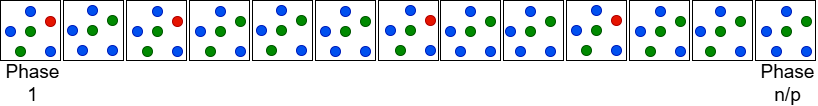
\includegraphics[scale=0.35]{proof2.png}
% \caption{Illustration of the system model}
\vspace{-2em}
\label{fig:SysModel}
\end{figure}
\end{frame}


\begin{frame}{Proof Intuition}
Consider the case of $|V_c|=2$:
\begin{itemize}
    \item At most $f$ phases can have Byzantine processes
    \item $(n/p)-f$ phases will have all correct processes
\end{itemize}
\vspace{-2em}
\begin{figure}[t]
\centering
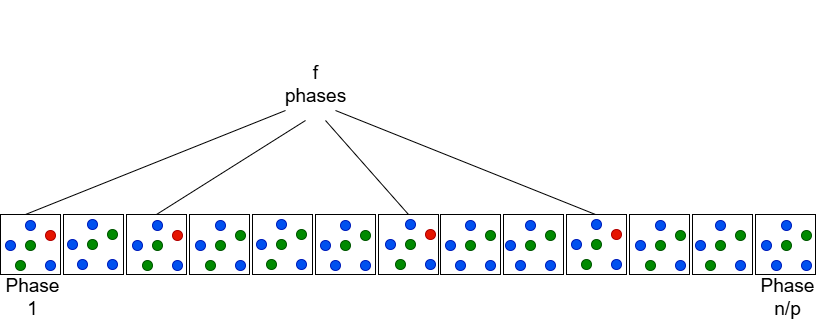
\includegraphics[scale=0.35]{proof3.png}
\end{figure}
\end{frame}


\begin{frame}{Proof Intuition}
Consider the case of $|V_c|=2$:
\begin{itemize}
    \item Pessimistic scenario: $f$ phases have Byzantine proposed values
    \item At least $((n/p)-f)/2$ phases will have winning value $1$, while the remaining phases will have the winning value $2$ (or vice versa).
\end{itemize}
\vspace{-2em}
\begin{figure}[t]
\centering
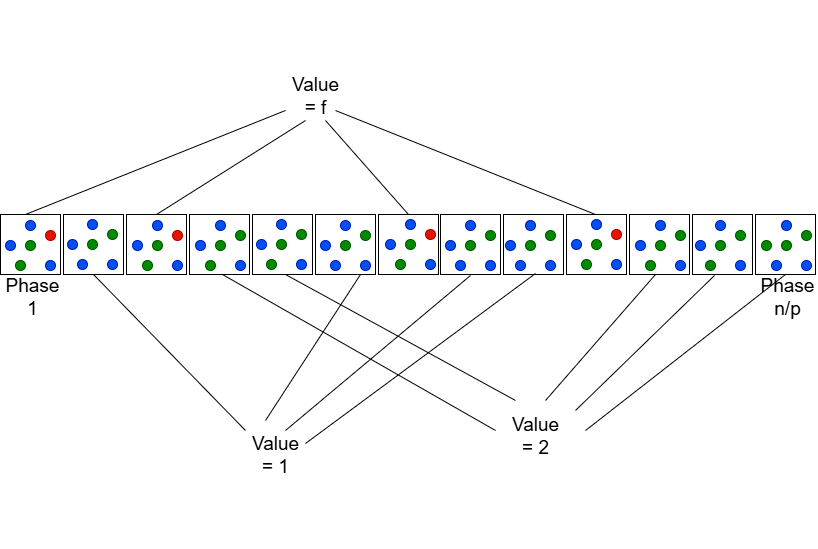
\includegraphics[scale=0.35]{proof4.png}
\end{figure}
\end{frame}


\begin{frame}{Proof Intuition}
Consider the case of $|V_c|=2$:
\begin{itemize}
    \item For consensus value to be $1$ or $2$, we need $mode$ to be either $1$ or $2$ i.e., $((n/p)-f)/2 > f$
    \item Solving for $f$ results in $f < n/(3p)$
    \item Extrapolating for all $|V_c|$, we derive $f< \frac{n}{(|V_c|+1)p}$
\end{itemize}
\vspace{-2em}
\begin{figure}[t]
\centering
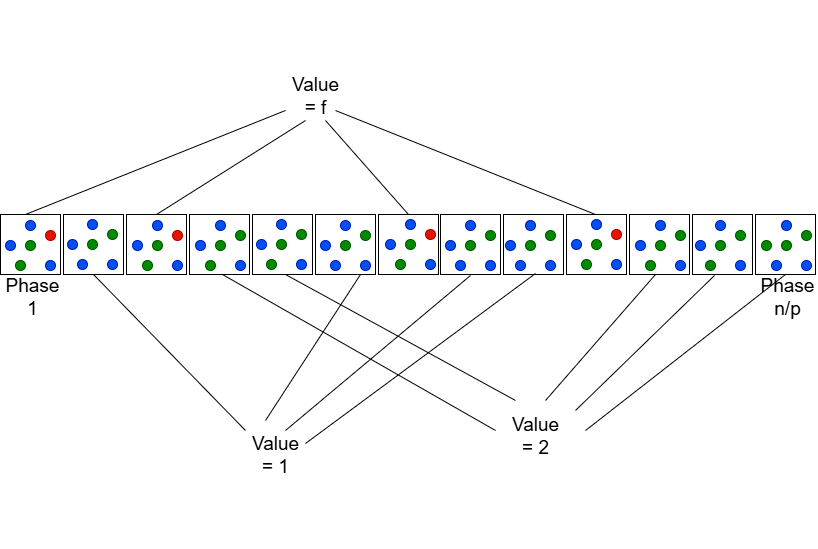
\includegraphics[scale=0.35]{proof4.png}
\end{figure}
\end{frame}




%------------------------------------------------

\begin{frame}{Conclusion}
\textbf{Summary:}
\begin{itemize}
  \item We introduced a \textbf{GPU-inspired Shared Memory Model} capturing unique architectural features.  
  \item Proposed a novel object, \textbf{\BVCAS}, enabling Byzantine-tolerant consensus.  
  \item Proved correctness and fault-resilience of our solution.  
\end{itemize}

\medskip
\textbf{Future Directions:}
\begin{itemize}
  \item Explore inter-block computations with multiple schedulers.  
  \item Investigate other fundamental problems under GPU-inspired models.  
  \item Study optimal resilience bounds achievable in this setting.  
\end{itemize}
\end{frame}


\begin{frame}
\vspace{2mm}
\centering
\Huge Thank you
\end{frame}


%---------------------------------------------------------
\section*{Extras}
%---------------------------------------------------------

%------------------------------------------------
\begin{frame}{Why We Need \BVCAS}
\begin{itemize}
  \item In Byzantine settings, simple registers are unsafe:
    \begin{itemize}
      \item A correct value can be overwritten by a faulty process.
      \item Leads to inconsistent states and broken agreement.
    \end{itemize}
  \item Sticky bits resist corruption but support only binary values.
  \item \BVCAS extends the idea to multi-valued consensus.
\end{itemize}
\end{frame}



\begin{frame}{Why Assumptions are Reasonable}
\begin{itemize}
  \item RR scheduling: baseline GPU behavior~\footfullcite{Jeon:springer:2025}.
  \item \Fwrite{} has constant cost (fits in one phase).
  \item \Fview{} may span multiple phases, consistent with GPU memory latency.
  \item Restricted access via objects is common for fault-tolerant designs.
\end{itemize}
\end{frame}

\begin{frame}{Weak Byzantine Consensus (WBC)}
\begin{definition}[\wbc] 
	Given $n$ processes, up to $f<n$ faulty, and correct values $V_c$, the following must hold:
	\begin{itemize}
		\item \textbf{Termination: } Every correct process must eventually decide.
		\item \textbf{Agreement: } All correct processes decide the same value.
	\end{itemize}
\end{definition}
\begin{itemize}
  \item Validity condition is dropped.
  \item Even if all correct processes propose the same value, the decision could be different.
\end{itemize}
\end{frame}

%------------------------------------------------
\begin{frame}{Common Value Byzantine Consensus (CVBC)}
\begin{theorem}[\cvbc] 
Proposed solution solves solves the \cvbc problem within $\Theta(n^2/p^2r)$ phases, for $f< \frac{n}{2p}$.
\end{theorem}
\end{frame}



\end{document}